\section{Performance Results}
\label{sec:results_scaling}

\begin{figure*}[t]
\centering
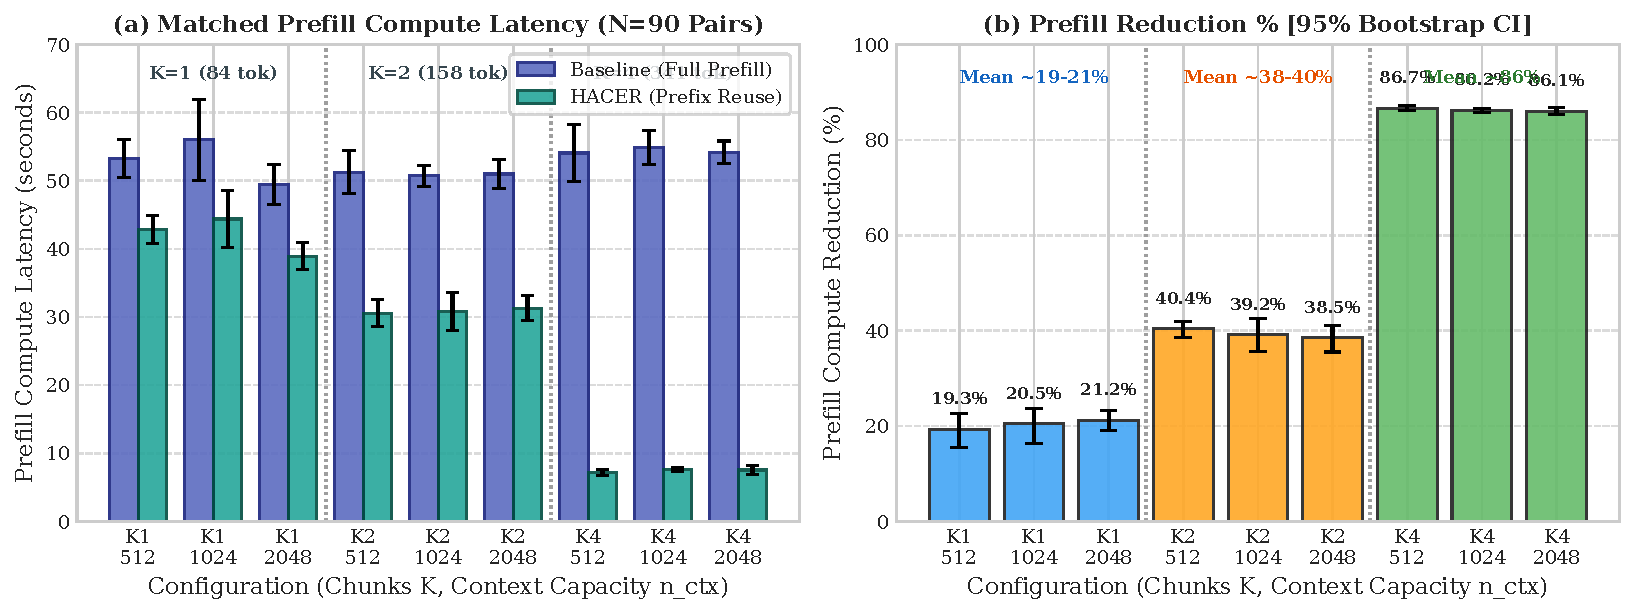
\includegraphics[width=\textwidth]{figures/fig2_scaling_latency_and_reduction.pdf}
\caption{\textbf{Physical Scaling Benchmark Results across 90 Matched Pairs (Xiaomi Redmi 12 5G).} (a) Absolute prompt prefill compute latency for baseline (cold) vs. HACER (reuse) across 9 configurations ($K \in \{1, 2, 4\}$ chunks, $n_{\text{ctx}} \in \{512, 1024, 2048\}$). (b) Prompt prefill compute reduction percentage with 95\% bootstrap confidence intervals, demonstrating consistent scaling across context sizes.}
\label{fig:scaling_results}
\end{figure*}

\begin{figure*}[t]
\centering
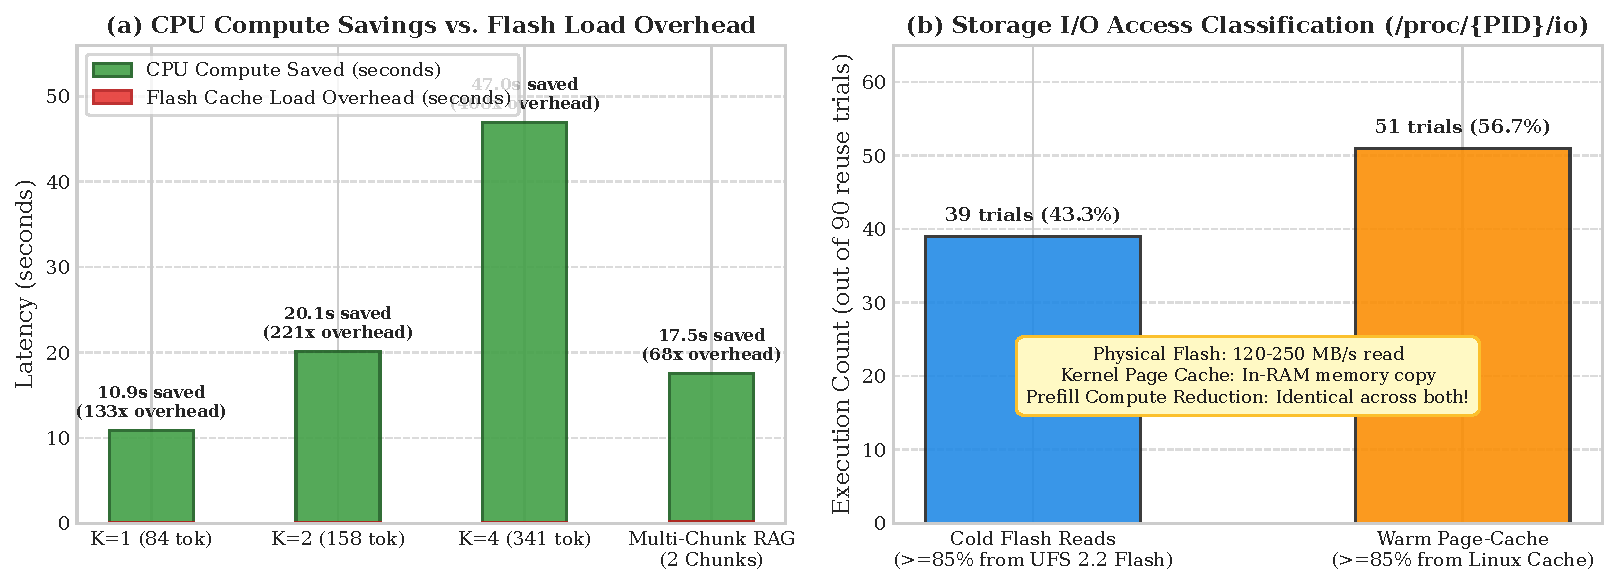
\includegraphics[width=\textwidth]{figures/fig3_io_and_storage_breakdown.pdf}
\caption{\textbf{Mobile Storage I/O and Compute Trade-Off Analysis.} (a) Comparison between CPU prefill execution time saved (10.4--47.3 seconds) and physical UFS 2.2 flash cache-load overhead (<0.35 seconds), demonstrating that CPU computation is orders of magnitude slower than mobile flash I/O. (b) Distribution of physical storage access modes across the 90 reuse trials (43.3\% cold flash reads vs. 56.7\% warm page cache hits), both yielding identical compute savings.}
\label{fig:storage_breakdown}
\end{figure*}

\subsection{Audit and Invariant Verification (182 Records)}
To ensure rigorous experimental reproducibility, all 182 raw trial records logged in \texttt{scaling\_trials.jsonl} were independently audited and verified prior to synthesis. The audit confirmed the following invariants:
\begin{enumerate}
    \item \textbf{Pairing and Quarantined Trials:} The log contains exactly 90 completed matched pairs (180 executions: 10 baseline and 10 reuse runs for each configuration C1 through C9). Exactly two incomplete executions were identified and quarantined:
    \begin{itemize}
        \item Pair \texttt{C5\_K2\_CTX1024\_rep1}: The reuse run succeeded, but the subsequent baseline run was interrupted by an incoming Android carrier focus dialog.
        \item Pair \texttt{C7\_K4\_CTX512\_rep2}: The reuse run succeeded, but the baseline run timed out due to background service preemption.
    \end{itemize}
    Both incomplete pairs were quarantined from paired statistical aggregation to prevent selection bias.
    \item \textbf{Prompt Invariance:} The canonical prompt SHA-256 digest was identical across all 182 records.
    \item \textbf{Zero Engine Truncations:} The engine truncation flag was false (\texttt{truncated == 0}) in 100\% of executions.
    \item \textbf{Deterministic Text Generation:} All 182 executions generated the byte-identical 35-token response string:
    \begin{quote}
    \small
    \texttt{"~Zephyr Dynamics was founded in 2011, the CLO is Jorge Fonseca, the AeroSense X7 battery lasts 72 hours, and the full-capacity tier"}
    \end{quote}
\end{enumerate}

\subsection{Physical Scaling Matrix Analysis}
Table~\ref{tab:scaling_matrix} summarizes the empirical scaling results across the nine evaluated configurations.

\begin{table*}[t]
\centering
\caption{\textbf{Physical Scaling Matrix Benchmark Results on Xiaomi Redmi 12 5G (90 Matched Pairs).}}
\label{tab:scaling_matrix}
\small
\begin{tabular}{lccccccc}
\toprule
\textbf{Configuration} & $K$ & $n_{\text{ctx}}$ & \textbf{Baseline Prefill (s)} & \textbf{Reuse Prefill (s)} & \textbf{Prefill Reduction [95\% CI]} & \textbf{Time Saved (s)} & \textbf{Wall Speedup} \\
\midrule
\textbf{C1\_K1\_CTX512} & 1 & 512 & $53.27 \pm 2.73$ & $42.85 \pm 2.00$ & \textbf{19.34\%} [15.50\%, 22.68\%] & $10.43 \pm 2.40$ & \textbf{1.19$\times$} \\
\textbf{C2\_K1\_CTX1024} & 1 & 1024 & $56.03 \pm 5.94$ & $44.39 \pm 4.16$ & \textbf{20.48\%} [16.28\%, 23.73\%] & $11.64 \pm 2.68$ & \textbf{1.22$\times$} \\
\textbf{C3\_K1\_CTX2048} & 1 & 2048 & $49.48 \pm 2.97$ & $38.93 \pm 1.98$ & \textbf{21.21\%} [19.10\%, 23.28\%] & $10.55 \pm 1.48$ & \textbf{1.21$\times$} \\
\midrule
\textbf{C4\_K2\_CTX512} & 2 & 512 & $51.28 \pm 3.12$ & $30.55 \pm 1.97$ & \textbf{40.37\%} [38.66\%, 41.94\%] & $20.72 \pm 1.44$ & \textbf{1.51$\times$} \\
\textbf{C5\_K2\_CTX1024} & 2 & 1024 & $50.73 \pm 1.58$ & $30.84 \pm 2.79$ & \textbf{39.16\%} [35.55\%, 42.59\%] & $19.89 \pm 2.03$ & \textbf{1.49$\times$} \\
\textbf{C6\_K2\_CTX2048} & 2 & 2048 & $51.01 \pm 2.08$ & $31.30 \pm 1.86$ & \textbf{38.53\%} [35.52\%, 41.08\%] & $19.71 \pm 1.81$ & \textbf{1.48$\times$} \\
\midrule
\textbf{C7\_K4\_CTX512} & 4 & 512 & $54.08 \pm 4.21$ & $7.18 \pm 0.40$ & \textbf{86.67\%} [86.18\%, 87.25\%] & $46.90 \pm 4.09$ & \textbf{3.60$\times$} \\
\textbf{C8\_K4\_CTX1024} & 4 & 1024 & $54.89 \pm 2.46$ & $7.56 \pm 0.28$ & \textbf{86.20\%} [85.73\%, 86.69\%] & $47.33 \pm 2.41$ & \textbf{3.65$\times$} \\
\textbf{C9\_K4\_CTX2048} & 4 & 2048 & $54.20 \pm 1.64$ & $7.55 \pm 0.61$ & \textbf{86.06\%} [85.25\%, 86.76\%] & $46.65 \pm 1.25$ & \textbf{3.27$\times$} \\
\bottomrule
\end{tabular}
\end{table*}

As illustrated in Figure~\ref{fig:scaling_results}, prompt prefill compute reduction scales monotonically with the number of cached prefix tokens:
\begin{itemize}
    \item \textbf{Single-Chunk Prefix ($K=1$, 84 Tokens Cached):} Yields a mean prefill reduction of $19.34\%$ to $21.21\%$ across context allocations, saving an average of $10.43$ to $11.64$ seconds of intensive CPU execution and delivering an end-to-end wall-clock speedup of $1.19\times$ to $1.22\times$.
    \item \textbf{Two-Chunk Prefix ($K=2$, 158 Tokens Cached):} Doubles the compute savings, achieving prefill reductions of $38.53\%$ to $40.37\%$ and saving approximately $20$ seconds per query, corresponding to a $1.48\times$ to $1.51\times$ wall speedup.
    \item \textbf{Four-Chunk Prefix ($K=4$, 341 Tokens Cached):} Ingesting nearly the entire prompt from cache (leaving only the 55 continuation and query tokens for online evaluation) yields prefill compute reductions of $86.06\%$ to $86.67\%$. Absolute prefill execution time drops from $54.89$~seconds down to $7.18$--$7.56$~seconds, saving over $46.9$~seconds of compute and delivering an end-to-end wall-clock speedup of up to \textbf{3.65$\times$}.
\end{itemize}

\subsection{Physical Storage I/O Profiling (Cold vs. Warm)}
A common concern in mobile KV caching is whether flash read latency diminishes compute gains. By capturing kernel I/O counters (\texttt{/proc/\{PID\}/io}), we classified all 90 reuse executions into physical access tiers (Figure~\ref{fig:storage_breakdown}b):
\begin{itemize}
    \item \textbf{Cold Flash Reads (39 trials, 43.3\%):} In these trials, $\ge 85\%$ of the session binary bytes were read directly from physical UFS 2.2 flash storage due to kernel page reclamation under system memory pressure.
    \item \textbf{Warm Page-Cache Hits (51 trials, 56.7\%):} In these trials, the session file remained resident in the Linux buffer cache.
\end{itemize}
Crucially, both cold and warm reuse executions produced statistically indistinguishable prefill compute latency reductions. Because the UFS 2.2 flash interface sustains read throughputs of 120--250~MB/s, loading a 40~MB session binary requires less than 250~ms—an overhead that is dwarfed by the 10.4 to 47.3~seconds of CPU prefill computation saved (Figure~\ref{fig:storage_breakdown}a).
